\section{复习}
\courseTime{Oct 17, 2022 \\ 5th}
上周被关了多久(笑)?上周是第一次线上上课,讲课特别不舒服。

上周讲了量子谐振子。这个科学问题来自氢分子的势能面,不管是定性还是定量,都要跟分子间相互作用打交道,包括弱相互作用、强相关作用等等。

在解离势能面最低点是平衡构型,这点能量与解离能量的差是解离能 $D_{\mathrm e}$。氢分子的势能也可以用单侧无限深势阱描述,类似束缚态。由品优波函数的条件,得到束缚态的超越方程 $\cot z = - \sqrt{\left(\frac{z_i}z\right)^2 - 1}$,解之得离散化的能量 $\{z_i\}$。这个模型预测零点能,误差极大。所以我们知道,想要预测整体性质——零点能,需要在平衡位置接近真实势能,特别是平衡位置的曲率。

从平衡位置做泰勒展开,那么得到了抛物势 $V(x) = \frac12 m \omega x^2$,即谐振子模型。利用品优条件求解它,得到了量子化的解。最重要的品优条件是无穷远处不能发散,由此得到了 Hermite 方程、间隔的递推公式,其中的发散项让我们必须在某项截断它。最终解得零点能 $E_i = \hbar\omega\left(n + \frac12\right)$。相比于单侧无限深势阱,这个的势能形状更符合氢气的解离曲线。值得关注的是,能级间隔是相等的 $\Delta E = \hbar\omega$,当氢分子偏离平衡位置时,非谐振效应体现出来,只能描述低振动级别的振动态,这是谐振子模型无法描述的,而单侧无限深势阱区分了束缚态和解离态。

我们引入更符合真实的 Morse 势,其定义为
\begin{eqnarray}
    V(x) = D_{\mathrm e} \ee^{-a (r-r_\mathrm e)} ( \ee^{-a (r - r_\mathrm e)} - 2),
\end{eqnarray}
在平衡处 $r_\mathrm e$ 有最小值,在无穷远处为 0。Morse 势的薛定谔方程有解。
\begin{lstlisting}
(* 画出 Morse 势能的图 *)
Clear["Global`*"]
De = 1; \[Alpha] = 1; re = 1;
M[r_] := De (1 - Exp[-\[Alpha] (r - re)])^2
Plot[M[r], {r, 0, 5}]
\end{lstlisting}
\homework{\textbf{5.1} 比较谐振子与 Morse 势能函数,参考 JCP 1988, 88(7) 4535 ``The Morse oscillator in position space and phase space''}
越接近真实体系,薛定谔方程越难求解。从没有限制的自由粒子开始,到简单的势能(仅通过边界条件求解),到现在势能形状也接近真实物理。当势能复杂到无法解析求解时,便可以通过数值求解。
\homework{\textbf{5.1} (\emph{continued}) (选做)采用 Numerov 方法数值求解。见 Levin \emph{Quantum Chemistry} Sec 4.4 P70}

\chapter{粒子的转动与角动量}
为什么要学习转动,因为真实体系不止有平动,还有转动、振动等。

从基本公设出发,可以解薛定谔方程求出体系的波函数。对体系了解程度,在于波函数的精确程度,求解的困难程度在于势函数的复杂性。

前面解了那么多的体系,共同点是一维的。从一维拓展到二维,最简单的还是自由粒子,哈密顿算符
\begin{align}
    \hat H = -\frac{\hbar^2}{2m} \left(\pdv[2]{x} + \pdv[2]{y}\right),
\end{align}
那么薛定谔方程
\begin{align}
    \hat H \Psi(x,y) = E \Psi(x,y)
\end{align}
我们希望波函数可以分离变量,
\begin{align}
    \Psi(x,y) = X(x) Y(y), \label{eq:2dtrans_sepXY}
\end{align}
得到左右两边相互独立的式子,
\begin{align}
    \hat F(x) X(x) = \hat G(y) Y(y)
\end{align}
数学上可以证明上式等价于
\begin{align}
    &\hat F(x) X(x) = C, \\
    &\hat G(y) Y(y) = C. 
\end{align}

将 \eqref{eq:2dtrans_sepXY} 代回薛定谔方程,
\begin{align}
    -\frac{\hbar}{2m} \left(\pdv[2]x + \pdv[2]y\right) X(x) Y(y) &= E X(x) Y(y) \\
    -\frac{\hbar^2}{2m} Y(y) \pdv[2]x X(x) - \frac{\hbar^2}{2m} X(x) \pdv[2]y Y(y) &= E X(x) Y(y) \\
    -\underbrace{\frac{\hbar^2}{2m} \frac1{X(x)} \pdv[2]x X(x)}_{\text{只与 $x$ 有关}} - 
    \underbrace{\frac{\hbar^2}{2m} \frac1{Y(y)} \pdv[2]y Y(y)}_{\text{只与 $y$ 有关}} &= E,
\end{align}
物化上应该讲过这种变换,分离得到只与 $x$ 或 $y$ 有关的两项。

\section{环上运动的粒子}
\begin{figure}[tp]\centering
    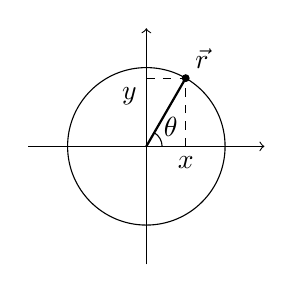
\begin{tikzpicture}[scale=1.0]
        % axis
        \draw[->] (-1.5,0) -- (1.5, 0);
        \draw[->] (0,-1.5) -- (0, 1.5);
        
        \draw (0,0) circle (1.0);
        \fill (0.5, 0.866) circle (0.05);
        \draw[dashed] (0.5, 0) -- (0.5, 0.866);
        \draw[dashed] (0, 0.866) -- (0.5, 0.866);
        \draw[thick] (0,0) -> (0.5, 0.866);
        \node[below] at (0.5, 0) {$x$};
        \node[below left] at (0.0, 0.866) {$y$};
        \node[above right] at (0.5, 0.866) {$\vec{r}$};
        \draw (0.2,0) arc (0:60:0.2);
        \node[above right] at (0.1,0) {$\theta$}; 
    
    \end{tikzpicture}
    \caption{环上的粒子}
\end{figure}
势函数
\begin{align}
    V(x,y) = \begin{cases}
        0, \quad & \sqrt{x^2 + y^2} = R,\\
        \infty, \quad &\sqrt{x^2 + y^2} \neq R, 
    \end{cases}
\end{align}
% 【讨论势能】
写出哈密顿量
\begin{align}
    \hat H = -\frac{\hbar^2}{2m} \left(\pdv[2]x + \pdv[2]y\right) + V(x,y)
\end{align}
此时无法分离变量 $\psi(x,y) \neq X(x) Y(y)$。如果将其变换到极坐标下,那么便可以分离变量,
\begin{align}
    \psi(r,\theta) = R(r) \Theta(\theta)
\end{align}
到底能否分离变量,求解完了才知道。

对波函数变换之后,还要把动能算符变换到极坐标下。这种变换相当于高中的难题,暴力求解比较麻烦,通常需要在求解开始时做非常巧妙的代换。尝试直接求解,首先,波函数的偏导不管在任何坐标下都是相等的,
\begin{align}
    \pdv[2]x \psi(x,y) = \pdv[2]{x} \psi(r,\theta),
\end{align}
用链式法则求解
\begin{align}
    &\pdv{\psi}{x} = \pdv{\psi}{r} \pdv{r}{x} + \pdv{\psi}{\theta} \pdv{\theta}{x},\\
    &\pdv{\psi}{y} = \pdv{\psi}{r} \pdv{r}{y} + \pdv{\psi}{\theta} \pdv{\theta}{y},
\end{align}
有几个显然的关系,
\begin{align}
    r^2 = x^2 + y^2, \quad \sin \theta = \frac xr,\quad \cos\theta = \frac yr,
\end{align}
径向对坐标的偏导,
\begin{align}
    \pdv{r}{x} = \pdv{x} \sqrt{x^2 + y^2} = \frac 12 \frac{2x}{\sqrt{x^2 + y^2}} = \frac xr = \cos\theta,
\end{align}
角度对坐标的偏导,利用 $\theta = \arccos \frac xr, x\in[0,\pi)$,
\begin{align}
    \pdv{\theta}{x} &= \pdv{x} \arccos \frac xr = -\frac1{\sqrt{1- \frac{x^2}{r^2}}} \left(\frac xr\right)^{\prime} \\
    &= -\frac ry \left(\frac 1r - \frac x{r^2} \frac xr\right) 
    = -\frac 1y \left(1 - \frac{x^2}{r^2}\right) \\
    &= -\frac{y}{r^2} = - \frac{\sin\theta} r, 
\end{align}
以上化简假设了 $\theta$ 在第一象限($x,y>0$),对于三四象限的角($y < 0$)需要加负号。
\begin{lstlisting}
(* 第一象限内的偏导 *)
D[ArcCos[x/Sqrt[x^2 + y^2]], x];
Simplify[%, Assumptions -> {x > 0, y > 0}]
>> -(y/(x^2 + y^2))
\end{lstlisting}

% 2022-10-17 08:54:22  Wenbin Fan @FDU
% 第二节课
% 下面得快一点了
那么对于波函数的导数
\begin{align}
    \pdv{\psi(x,y)}{x} = \cos\theta \pdv{\psi(r,\theta)}{r} - \frac{\sin\theta} r \pdv{\psi(r,\theta)}{\theta}, 
\end{align}
所以直接可给出
\begin{align}
    & \pdv{x} = \cos\theta \pdv{r} - \frac{\sin\theta}r \pdv{\theta},\\
    & \pdv{y} = \sin\theta \pdv{r} + \frac{\cos\theta}{r} \pdv{\theta},
\end{align}

再做二次偏导
\begin{align}
    \pdv[2]{\psi(x,y)}{x} = \pdv{x} \left(\cos\theta \frac{\psi}r - \frac{\sin\theta}r \pdv{\psi}{\theta}\right)
    \label{eq:polar_2nd_derv}
\end{align}
其中第一项
\begin{align}
    \pdv{x} \left(\cos\theta\pdv{\psi}{r}\right) 
    &= \pdv{\cos\theta}{x}\pdv{\psi}{r} + \cos\theta \pdv{x} \pdv{\psi}{r} \\
    &=\frac{\sin^2\theta}{r} \pdv{\psi}{r} + \cos\theta \left(\pdv[2]{\psi}{r} \pdv{r}{x} + \pdv[2]{\psi}{r}{\theta} \pdv{\theta}{x}\right) \\
    & = \frac{\sin^2\theta}{r} \pdv{\psi}{r} + \cos\theta \left( \cos\theta \pdv[2]{\psi}{r} - \frac{\sin\theta}{r} \pdv[2]{\psi}{r}{\theta}\right)
\end{align}
利用了
\begin{align}
    \pdv{x} \cos\theta = - \sin\theta \pdv{\theta}{x} = \frac{\sin^2\!\theta}{r},
\end{align}
第二项
\begin{align}
    \pdv{x} \left(\frac{\sin\theta}{r}\pdv{\psi}{x}\right) 
    &= - \frac{2\sin\theta \cos\theta}{r^2} \pdv{\psi}{\theta} + \frac{\sin\theta}r \left(\pdv[2]{\psi}{r}{\theta} \pdv{r}{x} + \pdv[2]{\psi}{\theta} \pdv{\theta}{x}\right)\\
    &=- \frac{2\sin\theta\cos\theta}{r^2} \pdv{\psi}{\theta} + \frac{\sin\theta \cos\theta}{r} \pdv[2]{\psi}{r}{\theta} - \frac{\sin^2\theta}{r^2} \pdv[2]{\psi}{\theta},
\end{align}
利用了
\begin{align}
    \pdv{x} \frac{\sin\theta}{r} = \pdv{x} \frac{y}{r^2} = \frac{-2y}{r^3} \pdv{r}{x} = -\frac{2\sin\theta\cos\theta}{r^2},
\end{align}
\begin{lstlisting}
(* 对 x 的二阶偏导,输出略 *)
D[\[Psi][Sqrt[x^2 + y^2], ArcCos[x/Sqrt[x^2 + y^2]]], {x, 2}];
Simplify[%, 
   Assumptions -> {x > 0, y > 0}] /. {y -> Sqrt[
    r^2 - r^2 Cos[\[Theta]]^2], x -> r Cos[\[Theta]]};
Simplify[%, Assumptions -> {r > 0, \[Theta] > 0, \[Theta] < Pi/2}]
\end{lstlisting}
于是
\begin{align}
    \pdv[2]{\psi(x,y)}{x}     
    &= \pdv{x} 
    \left(\cos\theta \pdv{\psi}{r} - \frac{\sin\theta}{r} \pdv{\psi}{\theta}\right) \\
    &= \cos^2\theta \pdv[2]{\psi}{r} - \frac{2\sin\theta\cos\theta}{r} \pdv[2]{\psi}{r}{\theta} + \frac{\sin^2\theta}{r^2} \pdv[2]{\psi}{\theta} \notag \\
    &\phantom{=} \quad + \frac{\sin^2\theta}{r} \pdv[2]{\psi}{r} + \frac{2\sin\theta\cos\theta}{r^2} \pdv{\psi}{\theta},
\end{align}
同理
\begin{align}
    \pdv[2]{\psi(x,y)}{y} &= \sin^2\!\theta \pdv[2]{\psi}{r} + \frac{2\sin\theta \cos\theta}{r} \pdv[2]{\psi}{r}{\theta} + \frac{\cos^2\theta}{r^2} \pdv[2]{\psi}{\theta} \notag\\
    &\phantom{=}\quad+ \frac{\cos^2\theta}{r} \pdv{\psi}{r} - \frac{2\sin\theta \cos\theta}{r^2} \pdv{\psi}{\theta}, 
\end{align}
于是 \eqref{eq:polar_2nd_derv} 为
\begin{align}
    \pdv[2]{\psi}{x} + \pdv[2]{\psi}{y} &= \pdv[2]{\psi}{r} + \frac1{r^2} \pdv[2]{\psi}{\theta} + \frac1r \pdv{\psi}{r} \\
    &=\pdv[2]{\psi}{r} + \frac1r \pdv{\psi}{r} + \frac1{r^2}\pdv[2]{\psi}{\theta}, 
\end{align}

最终哈密顿量写为
\begin{align}
    \hat H = - \frac{\hbar^2}{2m} \left(\pdv[2]{x} + \pdv[2]{y}\right) = -\frac{\hbar^2}{2m} \left(\pdv[2]{\psi}{r} + \frac1r \pdv{\psi}{r} + \frac1{r^2}\pdv[2]{\psi}{\theta}\right),
\end{align}
考虑本例中势能的特殊性,其径向部分为常数 $R$,因此哈密顿量仅与 $\theta$ 有关,
\begin{align}
    \hat H = - \frac{\hbar^2}{2mR^2} \pdv[2]{\theta} = -\frac{\hbar^2}{2I} \pdv[2]{\theta},
\end{align}
其中
\begin{eqnarray}
    I = m R^2
\end{eqnarray}
称之为\boldtext{转动惯量} momentum of inertia。%注意到 $\omega = \theta / t$,

薛定谔方程为
\begin{align}
    \hat H \varphi(\theta) &= E\varphi(\theta)\\
    - \frac{\hbar^2}{2I} \pdv[2]{\varphi}{\theta} &= E\varphi
\end{align}
整理得到
\begin{align}
    \pdv[2]{\varphi(\theta)}{\theta} + M^2 \varphi(\theta) = 0, \quad M^2 = \frac{2IE}{\hbar^2},
\end{align}
这是个二阶微分方程,设 $\varphi(\theta) = \ee^{s\theta}$,有
\begin{align}
    s^2 \ee^{s\theta} + M^2 \ee^{s\theta} = 0
\end{align}
得到
\begin{align}
    s^2 = - M^2 \Rightarrow s = \pm \ii M,
\end{align}
可得方程通解
\begin{align}
    \varphi(\theta) = A \ee^{\ii M\theta} + B \ee^{-\ii M \theta}
\end{align}
共有三个待求变量 $\{A, B, M\}$。

给出通解之后,利用边界条件得到量子化结果。在解无限深势阱的时候,利用了波函数连续、导数连续的条件。我们这里的二位极坐标体系,边界就是粒子转过 $2\pi$ 后又回来,所以有周期性边条件,
\begin{align}
    \varphi(\theta) = \varphi(\theta + 2\pi),
\end{align}
解得
\begin{align}
    \ee^{\ii M\, 2\pi} = 1 \Rightarrow M = 0, \pm 1, \pm 2, \cdots,
\end{align}
这里的 $M$ 称之为磁量子数 magnetic quantum number,从而可以解出能量
\begin{align}
    M^2 = \frac{2IE}{\hbar^2} \Rightarrow E = \frac{M^2\hbar^2} {2I} = \frac{M^2h^2} {8\pi^2 L},
\end{align}
知道了分子的转动惯量,就可以求出转动的精确谱、能量间隔。


讲到了转动,就必须要讲到角动量。角动量算符在经典力学中的定义为
\begin{align}
    \bm L = \bm r \times \bm p = \bm r \times m\bm v, 
\end{align}
对应的是右手定则。
分量形式
\begin{align}
    &L_x = y p_z - zp_y, \\
    &L_y = z p_x - x p_z, \\
    &L_z = x p_y - y p_x, 
\end{align}
微观体系中角动量是什么样的?

角动量的量子化 quantization,
\begin{align}
    \hat L_z = x \hat p_y - y \hat p_x = - \ii \hbar \left(x \pdv{y} - y \pdv{x}\right),
\end{align}
可以通过极坐标的变化求解出极坐标下的表达式,
\begin{align}
    \hat L_z = -\ii \hbar \pdv{\theta},
\end{align}
作为作业。
\homework{\textbf{5.2}  推导极坐标下的 $z$ 轴角动量算符 $\hat L_z$ 表达式。}
有个问题,我们说是量子化,其实直接用了动量算符的定义,但这是演绎,不是推导。如果在经典情况,$x$ 的位置无所谓,放在算符前后均可,以便跟量子情况相对于,实际上量子化不是直接加个 $\hat\cdot$ 得到的,角动量的量子化过程不具有普适性。

已经求出了环上粒子的通解,将
角动量算符作用到通解波函数上,
\begin{align}
    \hat L_z \varphi(\theta) \overset{?}{=} C\varphi(\theta),
\end{align}
会得到常数 $C$ 吗?不一定对吧,作用上去之后会有两个相反的系数 $\ii m$。这就很像动量算符和动能算符的关系,我们知道动量算符、动能算符是互易的,原则上可以共享同一个本征函数。
% \homework{\textbf{5.2} (\emph{continued}) 证明}

环上粒子的哈密顿量 $\hat H$ 和角动量 $\hat L_z$ 显然是对易的,所以它们可以共享相同的本征函数。通过构造本征函数,能求出通解,因为 $m$ 是任意的。并不要求角动量的本征函数是 $z$ 方向的。

量子力学基本假设第四条告诉我们,线性厄米算符给出来的本征函数是完备集,意思是任何函数都可以用这个完备集展开。二者共享本征函数的意思是,那么用这个共享的本征函数可以描述任何状态,无需只用一个或另一个,那么通解中的 $A$ 和 $B$ 可以去掉其中一个。剩下的一个代表它既是哈密顿量的本征函数,也是 $\hat L_z$ 的本征函数。

我们在实际的体系中,为什么要做这个事儿?正常来说,我们解薛定谔方程,通常只要基态能量,并不关心波函数是否是 $\hat L_z$ 的本征函数。在真实观测中,观测到的不仅是基态,还有各种的激发态。比如磁场下的分子,光谱中能看到各种磁量子数导致的细分。
% 【一大段讲述】
% 实际体系光谱,还有磁量子数。
% 状态波函数不仅是【】还是【】的本征函数,所以这个态是为了解磁量子数时光谱的细分【】。

在解氢原子体系时,能量只与 $n$ 有关。通过连带勒让德方程,还有 $m_l$ 等量子数。哈密顿算符是不区分 2p$_{-1}$、2p$_1$ 等,从实验中是可以同时准确观测到分量的。为什么能准确测量能量,同时在光谱中看到精确的磁量子数?因为哈密顿算符 $\hat H$ 和角动量 $\hat L$ 是对易的。动能和位置算符是不对易的,所以无法同时准确测量。

% 2022-10-17 13:24:54  Wenbin Fan @FDU
% 下午
\courseTime{下午}
简单回顾下早上的内容。想要了解任何感兴趣的体系,都要解薛定谔方程。目前的波函数都是不含时的,即定态方程。今天求解的势能函数是二维的,这是与之前最大的不同。通常二维势能难以在 Cartesian 空间求解,由合适的坐标变换可以简化求解过程。最契合环势能的坐标是极坐标,因此很自然地分离变量。

将环形势能变换到极坐标下,此时哈密顿量仅与 $\theta$ 有关,引入周期性边条件,得到磁量子数。随后演绎了角动量 $\hat l_z$ 的算符表示。

环运动的通解是两个本征函数的线性组合,包含了顺时针和逆时针旋转的组合。哈密顿算符和 $\hat l_z$ 是队医的,可以构造同时属于二者的本征函数完备集,所以可以把 $\varphi(\theta)$ 写成 $A \ee^{\ii m \varphi}$ 的形式。

接上午的求解。由归一化确定 $A$,
\begin{align}
    \int_0^{2\pi} \varphi^*(\theta) \varphi(\theta) \dd\theta = A^2 \int_{0}^{2\pi} \dd\theta = 2\pi A^2 = 1,
\end{align}
解之得
\begin{align}
    \varphi(\theta) = \frac{1}{\sqrt{2\pi}} \ee^{\ii m \theta}, \quad \rho(\theta) = |\varphi(\theta)|^2 = \frac1{2\pi},
\end{align}
因此波函数没有节点,任何地方的取值都是一样。我们现在求解的模型,都是希望贴近化学真实体系,与这个模型最相近的是苯环。
\homework{\textbf{5.2}  对于一维环形势箱,其能级为 
\begin{align}
    E_n = \frac{n^2 h^2}{8\pi^2 m R^2}, \quad n = 0, 1, 2, \cdots,
\end{align}
苯环的 $\pi$ 电子可近似看成是电子限制在一个环上的运动,$\pi$ 电子的半径是 \SI{1.4}{\angstrom},请以一维环形势箱的模型计算其最低激发能。

(以下选做)激发能的实验值是 \SI{2600}{\angstrom},讨论误差可能的来源。
}
随意讨论,真实的苯和离域电子的区别是什么。下周习题课,再下次求解熟悉的氢原子,我们现在从二维拓展到三维,为求解氢原子做准备。

\section{柱面上的粒子}
先讲一个简单的三维体系,(同学:球)真会找,找了个最难的。最简单的是自由粒子,三维自由粒子的算符,
\begin{align}
    \hat H = -\frac{\hbar^2}{2m} \left(\pdv[2]{x} + \pdv[2]{y} + \pdv[2]{z}\right), \quad \hat H \psi(x,y,z) = E \psi (x,y,z),
\end{align}
通过分离变量,可以解耦,求出来各个分量的波函数。

其次是无限深势阱的拓展,三维势能箱。比球简单一些的(安静),是圆柱啊!圆柱可以分离变量。接近真实的碳纳米管,这里以铜丝为例。
\homework{\textbf{5.3}  一圆柱体,长为 $l$、半径为 $R$,求解该圆柱体体系的能级,这里的势函数定义为
\begin{align}
    V(x,y,z) = \begin{cases}
        0, \quad &(x,y,z) \in \Omega,\\
        +\infty, \quad &(x,y,z) \notin \Omega,
    \end{cases}
\end{align}
其中
\begin{align}
    \Omega = \left\{(x,y,z) \, |\,  x^2+y^2 \leqslant R^2, 0\leqslant z\leqslant l\right\}. 
\end{align}
可参考徐昕老师 2000 年的文章 Jian-Lin Yao, Xin Xu, De-Yin Wu, et al, \emph{Chem. Commum.} 2000, 1627。
}
这些东西已经超越了课堂内容,但也确实是关于课堂内容触手可及的拓展。如果你会算这些习题,其实你已经可以做一些科研工作了。

现在计算机发达,很多人已经习惯了用 Gaussian 软件,用各种基函数展开波函数。
% 【】有助于掌握背后的物理。
化学从简单模型演变到复杂,越来越难算,主要源自于实验的精度越来越高。早期的实验,可控性很差,无法控制合成多孔材料、超分子等,无法控制形貌,只能通过宏观的温度等辅助合成。当近代实验操控能力增强,比如精准化学可以 100\% 操控反应物和产物,人们能制造出更精确的催化剂。这时计算化学便可以辅助实验,得到活性最高的形貌。
% 精确操控形状,什么形状有用?
% 【】【】【】【】【】

再复杂一点的,是球面上运动的粒子。

\section{球面上运动的粒子}
哈密顿量写出来
\begin{align}
    \hat H = -\frac{\hbar^2}{2m} \left(\pdv[2]x + \pdv[2]y + \pdv[2]z\right) + V(x,y,z),
\end{align}
其中势能
\begin{align}
    V(x,y,z) = \begin{cases}
        0, \quad &\sqrt{x^2+y^2+z^2} = r = R, \\
        \infty, \quad &\text{其它},
    \end{cases}
\end{align}
画出势能,坐标轴的定义是右手定则(四指从 $x$ 转向 $y$,大拇指指向 $z$),注意这里的 $\theta$ 是 $\bm r$ 与 $z$ 轴的夹角。
\begin{figure}
    \centering
    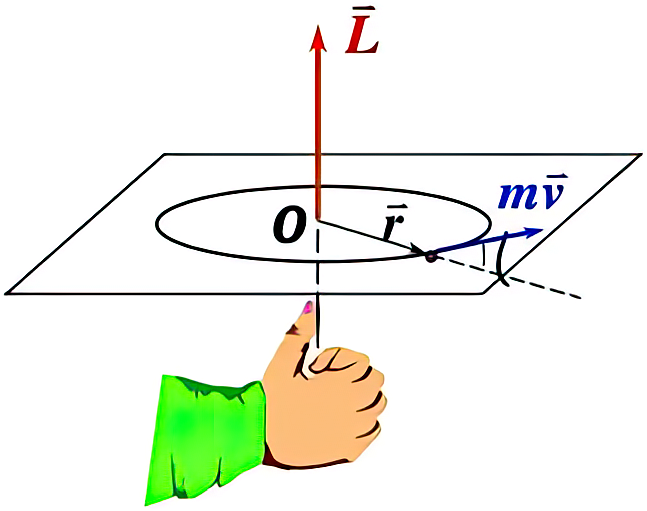
\includegraphics[width=3cm]{fig/angular_momentum.png}
    \caption{角动量方向}
    \label{fig:ang_direction}
\end{figure}

定义好坐标轴后,写出坐标映射
\begin{align}
    & x= r\,\sin\theta \, \cos\varphi, \\
    & y = r\,\sin\theta \, \sin\varphi, \\
    & z = r\,\cos\theta,
\end{align}
体积元变化
\begin{align}
    \Delta V = \Delta x \,\Delta y\, \Delta z,
\end{align}
\begin{figure}[tbp]
    \centering
    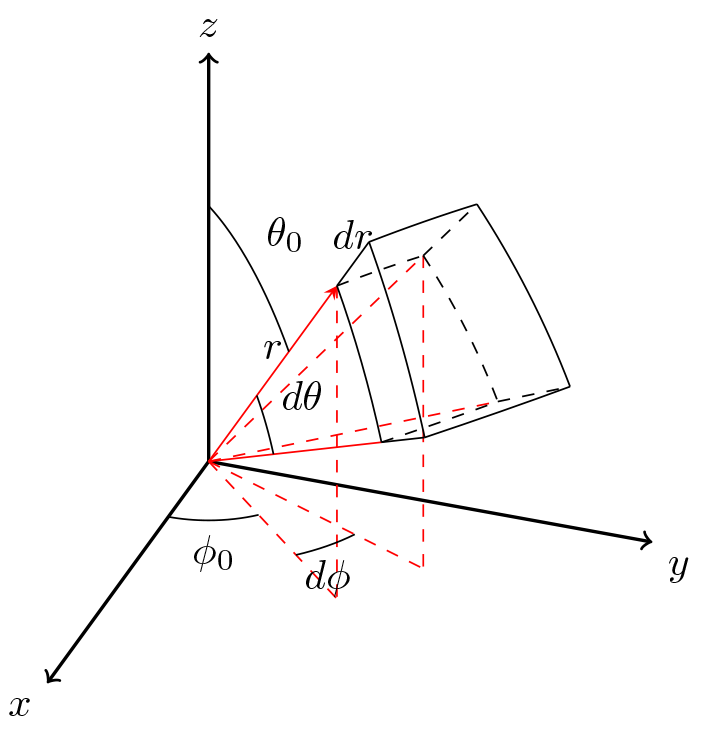
\includegraphics[width=4cm]{fig/3d_int_element.png}
    \caption{求坐标中的积分微元}
    % ref: https://blog.csdn.net/TanWaiwai_yy/article/details/104710427
\end{figure}
根据推导,有
\begin{align}
    \Delta V & =\dd s \, \dd r \\
    & = r \, \dd\theta \, r\sin\theta \, \dd\varphi \dd r \\
    & = r^2 \sin\theta \dd\theta \dd\varphi \dd r,
\end{align}
暴力推导的话,今天就别下课了。这里利用高级的数学方法,即利用 Jacob 矩阵来变换坐标系,
\begin{align}
    J = 
    \begin{pmatrix}
    \pdv{x}{r} & \pdv{x}{\theta} & \pdv{x}{\varphi} \\
    \pdv{y}{r} & \pdv{y}{\theta} & \pdv{y}{\varphi} \\
    \pdv{z}{r} & \pdv{z}{\theta} & \pdv{z}{\varphi}
    \end{pmatrix}, \quad 
    \begin{pmatrix}
        \pdv{r} \\ \pdv{\theta} \\ \pdv{\varphi}
    \end{pmatrix}
    = J 
    \begin{pmatrix}
        \pdv{x} \\ \pdv{y} \\ \pdv{z}
    \end{pmatrix},
\end{align}
直接得到结果,动能算符在极坐标下的表述,
\begin{align}
    \hat T = - \frac{\hbar^2}{2m} \left(
        \pdv[2]r + \frac2r \pdv{r} + \frac1{r^2} \hat \Lambda^2
    \right),
\end{align}
其中
\begin{align}
    \hat \Lambda^2 &= \frac1{\sin^2\theta} \pdv[2]{\varphi} + \frac1{\sin\theta} \pdv{\theta} \left(\sin\theta \pdv{\theta}\right) \\
    & = \frac1{\sin^2\theta} \pdv[2]{\varphi} + \cot\theta \pdv{\theta} + \pdv[2]{\theta},
\end{align}
这个算符 $\hat \Lambda$ 包含了动能中所有角度部分的能量,即角动量相关的能量,它一定与角动量相关。接下来很自然地考虑,三维的角动量如何考虑?

我们已经给出了二维的角动量,角动量的方向向外,沿着第三个坐标轴 $z$。角动量算符
\begin{align}
    \bm L = \bm r \times \bm p = \bm r \times m \bm v,
\end{align}
三个分量为
\begin{align}
    &\hat L_x = -\ii\hbar \left(y \pdv{z} - z \pdv{y}\right), \\
    &\hat L_y = -\ii\hbar \left(z \pdv{y} - y \pdv{z}\right), \\
    &\hat L_z = -\ii\hbar \left(x \pdv{y} - y \pdv{x}\right),
\end{align}
% 【还有两个式子没列上】
回顾两个例子中的解,
\begin{alignat}{2}
    &\text{二维极坐标} \quad &&\hat L_z = -\ii\hbar \pdv{\theta}, \\
    &\text{三维极坐标} \quad && \hat L_z = -\ii\hbar \pdv{\varphi},
\end{alignat}
% 【这里角动量分量好像不太对耶】
\homework{\textbf{5.4} 证明 
\begin{align}
    \hat L_x = -\ii\hbar \left(
        \sin\varphi \pdv{\theta} + \cot\theta \cos\varphi \pdv{\varphi}
    \right), \\
    \hat L_y = -\ii\hbar \left(
        \cos\varphi \pdv{\theta} - \cot\theta \sin\varphi \pdv{\varphi}
    \right),
\end{align}
并且利用
\begin{align}
    \hat L = \hat L_x \bm i + \hat L_y \bm j + \hat L_z \bm k
\end{align}
推导
\begin{align}
    \hat L^2 &= \hat L_x^2 + \hat L_y^2 + \hat L_z^2 \\&= -\hbar^2 \left(
        \frac1{\sin^2\theta} \pdv[2]{\varphi} + \cot\theta \pdv{\theta} + \pdv[2]{\theta}
    \right) \\
    &= -\hbar^2 \Lambda^2,
\end{align}
}

% 【推导 theta varphi 相关的式子】
% 【必须求解耦合的方程了】
% 当前体系的哈密顿量,
% \begin{align}
%     \hat H = -\frac{\hbar^2}{2mR^2} \hat\Lambda^2 = \frac1{2mR^2} \hat L^2 = - \frac1{2I},
% \end{align}
薛定谔方程
\begin{align}
    -\frac{\hbar^2}{2mR^2} \hat \Lambda^2 Y(\theta,\varphi) = E Y(\theta, \varphi), 
\end{align}
% 2022-10-17 14:24:07  Wenbin Fan @FDU
% 最后一节啦!
径向部分的偏导全部为 0,那么能否分离变量?
\begin{align}
    Y(\theta,\varphi) \overset{?}{=} \Theta(\theta) \Phi(\varphi),
\end{align}
尝试分离后代回,
\begin{align}
    \hat \Lambda^2  \Theta(\theta) \Phi(\varphi) + M^2  \Theta(\theta) \Phi(\varphi) = 0,
\end{align}
把 $\hat \Lambda^2$ 的定义代入,
\begin{align}
    \left(\frac1{\sin^2\theta} \pdv[2]{\varphi} + \cot\theta \pdv{\theta} + \pdv[2]{\theta}\right) \Theta(\theta) \Phi(\varphi) + M^2  \Theta(\theta) \Phi(\varphi) = 0, \notag\\
    \frac{\Theta(\theta)}{\sin^2\theta} \pdv[2]{\varphi} \Psi(\varphi) + \cot\theta \Psi(\varphi) \pdv{\theta} \Theta(\theta) + \Psi(\varphi) \pdv[2]{\theta} \Theta(\theta) + M^2 \Theta(\theta) \Psi(\varphi) = 0,
\end{align}
两边同时除以 $\Theta(\theta) \Phi(\varphi)$,
\begin{align}
    \frac{1}{\sin^2\theta \Psi(\varphi)} \pdv[2]{\varphi} \Psi(\varphi) + \frac{\cot\theta}{\Theta(\theta)} \pdv{\theta} \Theta(\theta) + \frac1{\Theta(\theta)} \pdv[2]{\theta} \Theta(\theta) + M^2 &= 0 \notag\\
    \underbrace{\frac{1}{\Psi(\varphi)} \pdv[2]{\varphi} \Psi(\varphi)}_{\varphi} 
    + 
    \underbrace{\frac{\sin\theta\,\cos\theta}{\Theta(\theta)} \pdv{\theta} \Theta(\theta) + \frac {\sin^2\theta}{\Theta(\theta)} \pdv[2]{\theta} \Theta(\theta) + M^2 \sin^2\theta}_{\theta}
    &= 0,
\end{align}
第一项只跟 $\varphi$ 有关,后面三项只跟 $\theta$ 有关,所以可以分开,分别移动到等号两端
\begin{align}
    \frac{1}{\Psi(\varphi)} \pdv[2]{\varphi} \Psi(\varphi) = - \left[
        \frac{\sin\theta\,\cos\theta}{\Theta(\theta)} \pdv{\theta} \Theta(\theta) + \frac {\sin^2\theta}{\Theta(\theta)} \pdv[2]{\theta} \Theta(\theta) + M^2 \sin^2\theta
    \right]
    \label{eq:sphere_surface_sep_done}
\end{align}
令左侧等于常数 $N$
\begin{align}
    \frac{1}{\Psi(\varphi)} \pdv[2]{\varphi} \Psi(\varphi) = N \Rightarrow  \pdv[2]{\varphi} \Psi(\varphi) = N \Psi(\varphi), 
\end{align}
取 $\Psi(\varphi) = \ee^{s\varphi}$,当 $N>0$ 时,$s = \pm\sqrt N$,$\Psi(\varphi) = \ee^{\pm \sqrt N \varphi}$ 发散、非品优,舍弃。%【】【】【N<0】
当 $N<0$ 时,$s = \pm\ii\sqrt{-N}$,$\Psi(\varphi) = \ee^{\pm\ii\sqrt N}$。

设 $N = - m_l^2$,得到
\begin{align}
    \Psi(\varphi) = A \ee^{\ii m_l \varphi} + B \ee^{-\ii m_l \varphi},
\end{align}

% 【共同本征函数】
因为
$\hat L^2$ 与 $\hat L_z$ 的共同本征函数解,
\begin{align}
    \Psi(\varphi) = A \ee^{\ii m_l \varphi} = \frac1{\sqrt{2\pi}} \ee^{\ii m_l \varphi}, \quad m_l = 0, \pm1, \pm2, \cdots,
\end{align}
因为有共同的本征值,那么 \eqref{eq:sphere_surface_sep_done} 右侧 $\Theta$ 相关的项等于 $-m_l^2$,
\begin{align}
    - \left[
        \frac{\sin\theta\,\cos\theta}{\Theta(\theta)} \pdv{\theta} \Theta(\theta) + \frac {\sin^2\theta}{\Theta(\theta)} \pdv[2]{\theta} \Theta(\theta) + M^2 \sin^2\theta
    \right] = -m_l^2,
\end{align}
整理得
\begin{align}
    \sin\theta\cos\theta \pdv{\theta} \Theta(\theta) + \sin^2\theta \Theta(\theta) = (m_l^2 - M^2 \sin^2\theta) \Theta(\theta),
\end{align}
在以前求解的体系中,能量是完全量子化的,但是这里的 $\theta,\varphi$ 完全不是,因为二者的量子数相互有关系,关于 $\varphi$ 的量子数要代入到 $\theta$ 的求解中。

该方程的解称作\boldtext{连带勒让德多项式}。目前还是太复杂了些,做一些变量代换。首先三角函数看起来就很麻烦,替换掉,设 $x = \cos\theta$,则 $\Theta(\theta) = y(x)$,求这个代换的偏导数,
\begin{align}
    &\pdv{\theta}\Theta(\theta) = \pdv{y(x)}{x} \pdv{x}{\theta} = \pdv{y(x)}{x}(-\sin\theta),\\
    &\pdv[2]{\theta} \Theta(\theta ) = 
    -\cos \pdv{y(x)}{x} - \sin\theta \pdv[2]{y(x)}{x} \pdv{x}{\theta} \\
    &\phantom{\pdv[2]{\theta} \Theta(\theta )} = 
    -\cos \pdv{y(x)}{x} + \sin^2\theta \pdv[2]{y(x)}{x}, 
\end{align}
代换完了是
\begin{multline}
    - x(1-x^2) \pdv[2]{y(x)}{x} + (1-x^2) \left[
        -x \pdv{y(x)}{x} + (1-x^2) \pdv[2]{y(x)}{x}
    \right] \\= \left[m_l^2 - M^2(1-x^2)\right] y(x),
\end{multline}
观察到其中每一项都含有 $(1-x^2)$,两边同时除以它。按照导数的次数排列,有
\begin{align}
    (1-x^2) y''(x) - 2x\, y'(x) + \left(M^2 - \frac{ml^2}{1-x^2}\right) y(x) = 0.
    \label{eq:legendre_ordered} % 按导数次序排列的
\end{align}

现在还不能求解它,因为当 $x = \cos\theta = \pm1$ 时有奇点,必须先消除奇点。

\boldtext{(1) 消除奇点},当 $x = \pm 1$ 时,
\begin{align}
    y(x) = (1 - x^2)^n H(x),
\end{align}
书上会告诉你当 $n = \frac{|m_l|}2$ 时可以消除,那么为什么呢?我们从头开始推导这个结果,即直接把 $n$ 代回原式。求出偏导方便一些,
\begin{align}
    &\pdv{y(x)}{x} = -2n x (1-x^n)^{n-1} H_n(x) + (1-x^2)^n H'(x),
\end{align}
二阶偏导稍麻烦
\begin{align}
    \pdv[2]{y(x)}{x} &= -2n x \left[
        (1-x^2)^{n-1} - 2(n-1)x^2(1-x^2)^{n-2}
    \right]H(x)  \notag\\
    &\quad\quad
    - 2n x(1-x^2)^{n-1} H'(x) 
    - 2n x(1-x^2)^{n-1} H'(x) \notag\\
    &\quad\quad + (1-x^2)^n H''(x) \\
    & = \left[
        -2n (1-x^2)^{n-1} + 4n (n-1) x^2 (1-x^2)^{n-2}
    \right] H(x) \notag\\
    &\quad\quad - 4nx(1-x^2)^{n-1} H'(x) + 
    (1-x^2)^n H''(x)
\end{align}
这时候再代回原式 \eqref{eq:legendre_ordered}
\begin{multline}
    \left[
        -2n (1-x^2)^n + 4n(n-1) x^2 (1-x^2)^{n-1}
    \right] H(x) \\
    - 4nx(1-x^2)^n H'(x) + (1-x^2)^{n+1} H''(x) \\
    + 4nx^2 (1-x^2)^{n-1} H(x) 
    - 2x (1-x^2)^n H'(x) \\
    +\left[
        M^2 (1-x^2)^n - m_l^2 (1-x^2)^{n-1}
    \right] H(x) = 0,
\end{multline}
合并同类项,
\begin{multline}
    (1-x^2)^{n+1} H''(x) - 2x(2n+1) (1-x^2)^n H'(x) 
    \\+ 
    \left[
        -2n (1-x^2)^n + 4n^2 x^2 (1-x^2)^{n-1} - m_l^2 (1-x^2)^{n-1} + M^2 (1-x^2)^n
    \right] H(x) \\= 0
\end{multline}
再化简,
\begin{align}
    (1-x^2) H''(x) - 2x(2n+1) H'(x) + \left[
        -2n + \frac{4n^2x^2 - m_l^2}{1-x^2} + M^2
    \right] H(x) = 0
\end{align}
也就是当 $4n^2 = m_l^2$ 时,有
\begin{align}
    \frac{m_l^2 (x^2 - 1)}{1 - x^2} = - m_l^2,
\end{align}
令 $n = \frac{|m_l|}2$,即
\begin{align}
    y(x) = (1 - x^2)^{|m_l|/2} H(x),
\end{align}
有
\begin{align}
    (1-x^2) H''(x) - 2\left(|m_l| + 1\right)x \, H'(x) + \left(m^2 - m_l^2 - |m_l|\right) H(x) = 0. 
\end{align}

整个解法从头到尾写下来很累的,但是每一步都有逻辑。量子的教科书上都是这个结论,读者难以知道整个过程。

在学习特殊函数或者数学物理方程时,最有创造性的一点是一开始选什么样的初猜,即选择什么样的通解。球面上的粒子也是一样,从尝试分离变量开始,再到消奇点,很幸运有连带勒让德函数这个解。

% 2022-10-17 15:08:33  Wenbin Fan @FDU
% 快下课了 XD
% 这段求解过程好乏味……
下节课继续讲幂级数求解法。











